\documentclass[tikz,border=5pt]{standalone}
\usepackage{tikz}
\usetikzlibrary{arrows.meta}
\begin{document}
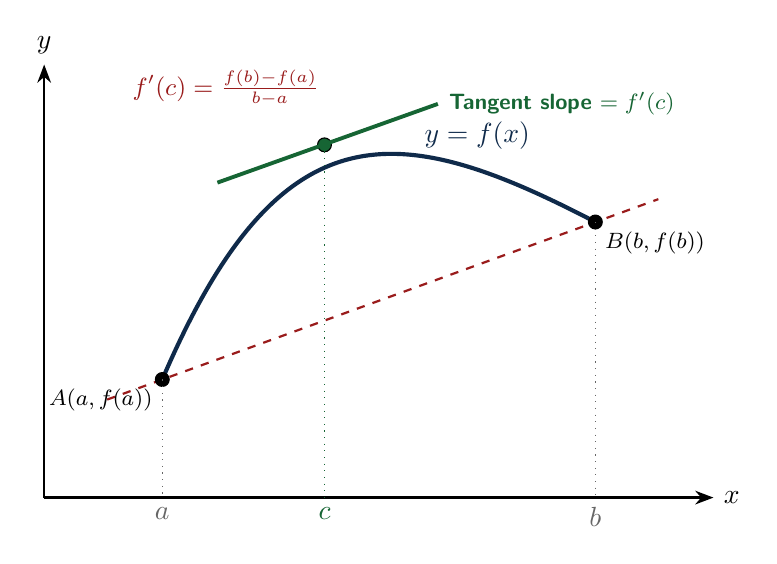
\begin{tikzpicture}[>=Stealth, scale=1.0]
  \definecolor{navyblue}{HTML}{0F2A4A}
  \definecolor{accentcrimson}{HTML}{991B1B}
  \definecolor{forestgreen}{HTML}{166534}

  % Axes
  \draw[thick, ->] (0,0) -- (8.5,0) node[right, font=\sffamily\bfseries] {$x$};
  \draw[thick, ->] (0,0) -- (0,5.5) node[above, font=\sffamily\bfseries] {$y$};

  % Points A(1, 1.5) and B(7, 3.5)
  \coordinate (A) at (1.5, 1.5);
  \coordinate (B) at (7.0, 3.5);

  % Function curve with a bump
  \draw[line width=1.5pt, navyblue] (1.5, 1.5) .. controls (3.0, 5.0) and (4.5, 4.8) .. (7.0, 3.5);
  \node[navyblue, font=\sffamily\bfseries] at (5.5, 4.6) {$y = f(x)$};

  % Secant line AB
  \draw[thick, dashed, accentcrimson] (0.8, 1.245) -- (7.8, 3.79);
  \draw[fill=black] (A) circle (2.5pt) node[below left, font=\sffamily\footnotesize\bfseries] {$A(a, f(a))$};
  \draw[fill=black] (B) circle (2.5pt) node[below right, font=\sffamily\footnotesize\bfseries] {$B(b, f(b))$};

  % Point C where derivative equals secant slope
  \coordinate (C) at (3.56, 4.48);
  \draw[fill=forestgreen] (C) circle (2.5pt);
  \draw[line width=1.4pt, forestgreen] (2.2, 4.0) -- (5.0, 5.0) node[right, font=\sffamily\footnotesize\bfseries] {Tangent slope $= f'(c)$};

  % Projections to x-axis
  \draw[dotted, black!60] (1.5, 1.5) -- (1.5, 0) node[below, font=\sffamily\bfseries] {$a$};
  \draw[dotted, black!60] (7.0, 3.5) -- (7.0, 0) node[below, font=\sffamily\bfseries] {$b$};
  \draw[dotted, forestgreen] (C) -- (3.56, 0) node[below, forestgreen, font=\sffamily\bfseries] {$c$};

  \node[anchor=west, font=\sffamily\small\bfseries, accentcrimson] at (1.0, 5.2) 
    {$f'(c) = \frac{f(b) - f(a)}{b - a}$};
\end{tikzpicture}
\end{document}